\documentclass{ximera}

\title{Unit I: Ax = b and the Four Subspaces}

\begin{document}

\begin{abstract}
  Unit 1 MIT OCW Linear Algebra
\end{abstract}\maketitle

\vspace{2 mm}

\begin{center}
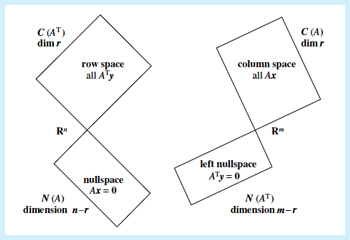
\includegraphics{Unit_1_WIDE.jpg}
The big picture of linear algebra: Four Fundamental Subspaces.
\end{center}

\noindent
Mathematics is a tool for describing the world around us. Linear equations give some of the simplest descriptions, and systems of linear equations are made by combining several descriptions.

\vspace{5 mm}

\noindent
In this unit we write systems of linear equations in the matrix form Ax = b. We explore how the properties of A and b determine the solutions x (if any exist) and pay particular attention to the solutions to Ax = 0. For a given matrix A we ask which b can be written in the form Ax.

\end{document}

